% Created 2021-08-04 on 12:08
% Intended LaTeX compiler: pdflatex
\documentclass[12pt]{article}

%%%% settings when exporting code %%%% 

\usepackage{listings}
\lstdefinestyle{code-small}{
backgroundcolor=\color{white}, % background color for the code block
basicstyle=\ttfamily\small, % font used to display the code
commentstyle=\color[rgb]{0.5,0,0.5}, % color used to display comments in the code
keywordstyle=\color{black}, % color used to highlight certain words in the code
numberstyle=\ttfamily\tiny\color{gray}, % color used to display the line numbers
rulecolor=\color{black}, % color of the frame
stringstyle=\color[rgb]{0,.5,0},  % color used to display strings in the code
breakatwhitespace=false, % sets if automatic breaks should only happen at whitespace
breaklines=true, % sets automatic line breaking
columns=fullflexible,
frame=single, % adds a frame around the code (non,leftline,topline,bottomline,lines,single,shadowbox)
keepspaces=true, % % keeps spaces in text, useful for keeping indentation of code
literate={~}{$\sim$}{1}, % symbol properly display via latex
numbers=none, % where to put the line-numbers; possible values are (none, left, right)
numbersep=10pt, % how far the line-numbers are from the code
showspaces=false,
showstringspaces=false,
stepnumber=1, % the step between two line-numbers. If it's 1, each line will be numbered
tabsize=1,
xleftmargin=0cm,
emph={anova,apply,class,coef,colnames,colNames,colSums,dim,dcast,for,ggplot,head,if,ifelse,is.na,lapply,list.files,library,logLik,melt,plot,require,rowSums,sapply,setcolorder,setkey,str,summary,tapply},
aboveskip = \medskipamount, % define the space above displayed listings.
belowskip = \medskipamount, % define the space above displayed listings.
lineskip = 0pt} % specifies additional space between lines in listings
\lstset{style=code-small}
%%%% packages %%%%%

\usepackage[utf8]{inputenc}
\usepackage[T1]{fontenc}
\usepackage{lmodern}
\usepackage{textcomp}
\usepackage{color}
\usepackage{graphicx}
\usepackage{grffile}
\usepackage{wrapfig}
\usepackage{rotating}
\usepackage{longtable}
\usepackage{multirow}
\usepackage{multicol}
\usepackage{changes}
\usepackage{pdflscape}
\usepackage{geometry}
\usepackage[normalem]{ulem}
\usepackage{amssymb}
\usepackage{amsmath}
\usepackage{amsfonts}
\usepackage{dsfont}
\usepackage{array}
\usepackage{ifthen}
\usepackage{hyperref}
\usepackage{natbib}
\RequirePackage{setspace} % to modify the space between lines - incompatible with footnote in beamer
\renewcommand{\baselinestretch}{1.1}
\geometry{top=1cm}
\usepackage{titlesec}
\usepackage{etoolbox}

\makeatletter
\patchcmd{\ttlh@hang}{\parindent\z@}{\parindent\z@\leavevmode}{}{}
\patchcmd{\ttlh@hang}{\noindent}{}{}{}
\makeatother
\RequirePackage{colortbl} % arrayrulecolor to mix colors
\definecolor{myorange}{rgb}{1,0.2,0}
\definecolor{mypurple}{rgb}{0.7,0,8}
\definecolor{mycyan}{rgb}{0,0.6,0.6}
\newcommand{\lightblue}{blue!50!white}
\newcommand{\darkblue}{blue!80!black}
\newcommand{\darkgreen}{green!50!black}
\newcommand{\darkred}{red!50!black}
\definecolor{gray}{gray}{0.5}
\hypersetup{
citecolor=[rgb]{0,0.5,0},
urlcolor=[rgb]{0,0,0.5},
linkcolor=[rgb]{0,0,0.5},
}
\newenvironment{note}{\small \color{gray}\fontfamily{lmtt}\selectfont}{\par}
\newenvironment{activity}{\color{orange}\fontfamily{qzc}\selectfont}{\par}
\RequirePackage{pifont}
\RequirePackage{relsize}
\newcommand{\Cross}{{\raisebox{-0.5ex}%
{\relsize{1.5}\ding{56}}}\hspace{1pt} }
\newcommand{\Valid}{{\raisebox{-0.5ex}%
{\relsize{1.5}\ding{52}}}\hspace{1pt} }
\newcommand{\CrossR}{ \textcolor{red}{\Cross} }
\newcommand{\ValidV}{ \textcolor{green}{\Valid} }
\usepackage{stackengine}
\usepackage{scalerel}
\newcommand\Warning[1][3ex]{%
\renewcommand\stacktype{L}%
\scaleto{\stackon[1.3pt]{\color{red}$\triangle$}{\tiny\bfseries !}}{#1}%
\xspace
}
\newcommand\Rlogo{\textbf{\textsf{R}}\xspace} %
\RequirePackage{fancyvrb}
\DefineVerbatimEnvironment{verbatim}{Verbatim}{fontsize=\small,formatcom = {\color[rgb]{0.5,0,0}}}
\RequirePackage{enumitem} % better than enumerate
\RequirePackage{epstopdf} % to be able to convert .eps to .pdf image files
\RequirePackage{capt-of} %
\RequirePackage{caption} % newlines in graphics
\RequirePackage{tikz-cd} % graph
\RequirePackage{booktabs} % for nice lines in table (e.g. toprule, bottomrule, midrule, cmidrule)
\RequirePackage{amsmath}
\RequirePackage{algorithm}
\RequirePackage[noend]{algpseudocode}
\RequirePackage{dsfont}
\RequirePackage{amsmath,stmaryrd,graphicx}
\RequirePackage{prodint} % product integral symbol (\PRODI)
\usepackage{ifthen}
\usepackage{xifthen}
\usepackage{xargs}
\usepackage{xspace}
\newcommand\defOperator[7]{%
\ifthenelse{\isempty{#2}}{
\ifthenelse{\isempty{#1}}{#7{#3}#4}{#7{#3}#4 \left#5 #1 \right#6}
}{
\ifthenelse{\isempty{#1}}{#7{#3}#4_{#2}}{#7{#3}#4_{#1}\left#5 #2 \right#6}
}
}
\newcommand\defUOperator[5]{%
\ifthenelse{\isempty{#1}}{
#5\left#3 #2 \right#4
}{
\ifthenelse{\isempty{#2}}{\underset{#1}{\operatornamewithlimits{#5}}}{
\underset{#1}{\operatornamewithlimits{#5}}\left#3 #2 \right#4}
}
}
\newcommand{\defBoldVar}[2]{
\ifthenelse{\equal{#2}{T}}{\boldsymbol{#1}}{\mathbf{#1}}
}
\newcommandx\Esp[2][1=,2=]{\defOperator{#1}{#2}{E}{}{\lbrack}{\rbrack}{\mathbb}}
\newcommandx\Prob[2][1=,2=]{\defOperator{#1}{#2}{P}{}{\lbrack}{\rbrack}{\mathbb}}
\newcommandx\Qrob[2][1=,2=]{\defOperator{#1}{#2}{Q}{}{\lbrack}{\rbrack}{\mathbb}}
\newcommandx\Var[2][1=,2=]{\defOperator{#1}{#2}{V}{ar}{\lbrack}{\rbrack}{\mathbb}}
\newcommandx\Cov[2][1=,2=]{\defOperator{#1}{#2}{C}{ov}{\lbrack}{\rbrack}{\mathbb}}
\newcommandx\Binom[2][1=,2=]{\defOperator{#1}{#2}{B}{}{(}{)}{\mathcal}}
\newcommandx\Gaus[2][1=,2=]{\defOperator{#1}{#2}{N}{}{(}{)}{\mathcal}}
\newcommandx\Wishart[2][1=,2=]{\defOperator{#1}{#2}{W}{ishart}{(}{)}{\mathcal}}
\newcommandx\Likelihood[2][1=,2=]{\defOperator{#1}{#2}{L}{}{(}{)}{\mathcal}}
\newcommandx\logLikelihood[2][1=,2=]{\defOperator{#1}{#2}{\ell}{}{(}{)}{}}
\newcommandx\Information[2][1=,2=]{\defOperator{#1}{#2}{I}{}{(}{)}{\mathcal}}
\newcommandx\Score[2][1=,2=]{\defOperator{#1}{#2}{S}{}{(}{)}{\mathcal}}
\newcommandx\Vois[2][1=,2=]{\defOperator{#1}{#2}{V}{}{(}{)}{\mathcal}}
\newcommandx\IF[2][1=,2=]{\defOperator{#1}{#2}{IF}{}{(}{)}{\mathcal}}
\newcommandx\Ind[1][1=]{\defOperator{}{#1}{1}{}{(}{)}{\mathds}}
\newcommandx\Max[2][1=,2=]{\defUOperator{#1}{#2}{(}{)}{min}}
\newcommandx\Min[2][1=,2=]{\defUOperator{#1}{#2}{(}{)}{max}}
\newcommandx\argMax[2][1=,2=]{\defUOperator{#1}{#2}{(}{)}{argmax}}
\newcommandx\argMin[2][1=,2=]{\defUOperator{#1}{#2}{(}{)}{argmin}}
\newcommandx\cvD[2][1=D,2=n \rightarrow \infty]{\xrightarrow[#2]{#1}}
\newcommandx\Hypothesis[2][1=,2=]{
\ifthenelse{\isempty{#1}}{
\mathcal{H}
}{
\ifthenelse{\isempty{#2}}{
\mathcal{H}_{#1}
}{
\mathcal{H}^{(#2)}_{#1}
}
}
}
\newcommandx\dpartial[4][1=,2=,3=,4=\partial]{
\ifthenelse{\isempty{#3}}{
\frac{#4 #1}{#4 #2}
}{
\left.\frac{#4 #1}{#4 #2}\right\rvert_{#3}
}
}
\newcommandx\dTpartial[3][1=,2=,3=]{\dpartial[#1][#2][#3][d]}
\newcommandx\ddpartial[3][1=,2=,3=]{
\ifthenelse{\isempty{#3}}{
\frac{\partial^{2} #1}{\partial #2^2}
}{
\frac{\partial^2 #1}{\partial #2\partial #3}
}
}
\newcommand\Real{\mathbb{R}}
\newcommand\Rational{\mathbb{Q}}
\newcommand\Natural{\mathbb{N}}
\newcommand\trans[1]{{#1}^\intercal}%\newcommand\trans[1]{{\vphantom{#1}}^\top{#1}}
\newcommand{\independent}{\mathrel{\text{\scalebox{1.5}{$\perp\mkern-10mu\perp$}}}}
\newcommand\half{\frac{1}{2}}
\newcommand\normMax[1]{\left|\left|#1\right|\right|_{max}}
\newcommand\normTwo[1]{\left|\left|#1\right|\right|_{2}}
\newcommand\Veta{\boldsymbol{\eta}}
\newcommand\VX{\mathbf{X}}
\newcommand\sample{\chi}
\newcommand\Hspace{\mathcal{H}}
\newcommand\Tspace{\mathcal{T}}
\author{Brice Ozenne}
\date{\today}
\title{Inverse probability of censoring weighting (IPCW) for linear regression}
\hypersetup{
 colorlinks=true,
 pdfauthor={Brice Ozenne},
 pdftitle={Inverse probability of censoring weighting (IPCW) for linear regression},
 pdfkeywords={},
 pdfsubject={},
 pdfcreator={Emacs 27.1 (Org mode 9.4.5)},
 pdflang={English}
 }
\begin{document}

\maketitle

\section{Principle}
\label{sec:org6b5d322}

Inverse probability of censoring weighting (IPCW) is a method able to
handle informative drop-out. Intuitively, in presence of informative
drop-out a complete case analysis is a biased approach as individuals
with complete data are not representative of the population. However
with an appropriate re-weighting of the individuals with complete
data, we can "re-balance" our sample and make it representative of the
population. To do so, we divide the population into sub-populations
and attribute weights to individuals who did not drop-out inversely
proportional to the frequency of the drop-out in the
sub-population. Thanks to the weights, individuals who did not
drop-out "represent" the individuals who dropped-out. Thus, overall,
the weighted sample is representative of the population.



\section{Illustrative example}
\label{sec:org88ba9e6}

Consider a study were we follow depressed individual over time. They
have a baseline measurement, then are given a treatment, and then have
a follow-up measurement. We would like to assess the treatment effect
in term of depression score \footnote{:To simplfy, there is no control
group - we assume that without treatment the depression score would be
constant.}. The population of interest contain severely and moderately
depressed individuals; the treatment may work differently in each
sub-population. Unfortunately, some study participants dropped-out and
it seems that they are more likely to drop-out when they are severaey
depressed.

\clearpage

We can simulate such a dataset using the following function:
\lstset{language=r,label= ,caption= ,captionpos=b,numbers=none}
\begin{lstlisting}
simTrial <- function(n, rho, dmu, pC){
  require(mvtnorm)
  require(data.table)
  ## simulate data
  Sigma <- 10^2*matrix(c(1,rho,rho,1),2,2)
  ## gather into dataset
  M.Ym <- rmvnorm(n, mean = c(50, 50-dmu[1]), sigma = Sigma)
  M.Ys <- rmvnorm(n, mean = c(75, 75-dmu[2]), sigma = Sigma)
  dtL <- rbind(
    data.table(id = 1:n, mdd = "moderate", time = "T1", Y = M.Ym[,1]),
    data.table(id = 1:n, mdd = "moderate", time = "T2", Y = M.Ym[,2]),
    data.table(id = n+(1:n), mdd = "severe", time = "T1", Y = M.Ys[,1]),
    data.table(id = n+(1:n), mdd = "severe", time = "T2", Y = M.Ys[,2])
  )
  dtL$probaDO <- 0
  dtL[time=="T2", probaDO := ifelse(.SD$mdd=="moderate",pC[1],pC[2])]
  dtL[,dropout := rbinom(.N,prob=probaDO,size=1)]
  dtL[,Yobs:=Y]
  dtL[dropout==1,Yobs:=NA]
  dtL$probaDO <- NULL
  return(dtL)
}
set.seed(11)
dtL <- simTrial(n = 1000, rho = 0.8, dmu = c(25,50), pC = c(0.2,0.7))
print(dtL)
\end{lstlisting}

\begin{verbatim}
        id      mdd time        Y dropout     Yobs
   1:    1 moderate   T1 44.83259       0 44.83259
   2:    2 moderate   T1 30.34157       0 30.34157
   3:    3 moderate   T1 56.36308       0 56.36308
   4:    4 moderate   T1 64.63341       0 64.63341
   5:    5 moderate   T1 45.10048       0 45.10048
  ---                                             
3996: 1996   severe   T2 30.59793       1       NA
3997: 1997   severe   T2 18.97725       1       NA
3998: 1998   severe   T2 29.80266       1       NA
3999: 1999   severe   T2 30.26518       0 30.26518
4000: 2000   severe   T2 39.15797       0 39.15797
\end{verbatim}

Here we have simulated a two sub-populations of 1000, with a
correlation of 0.5 between baseline and follow-up . The treatment
effect is twice bigger for the severely depressed population but
individuals from this population are also much more likely to
drop-out. Overall the expected treatment effect is:
\lstset{language=r,label= ,caption= ,captionpos=b,numbers=none}
\begin{lstlisting}
(-25-50)/2
\end{lstlisting}

\begin{verbatim}
[1] -37.5
\end{verbatim}


\bigskip

Without drop-out, we could use a simple linear model to carry-out the analysis:
\lstset{language=r,label= ,caption= ,captionpos=b,numbers=none}
\begin{lstlisting}
dtW.oracle <- dcast(dtL, formula = id ~ time, value.var = "Y")
dtW.oracle$diff <- dtW.oracle$T2-dtW.oracle$T1
e.oracle <- lm(diff~1, data = dtW.oracle)
summary(e.oracle)$coef
\end{lstlisting}

\begin{verbatim}
             Estimate Std. Error   t value Pr(>|t|)
(Intercept) -37.35098  0.3141814 -118.8835        0
\end{verbatim}

leading to an estimate quite close to the true value.

\bigskip

With drop-out, a complete case analysis would lead to a biased
estimator. In this example, we can "see" that the estimated value is
far away from the true one (even when accouting for the uncertainty):
\lstset{language=r,label= ,caption= ,captionpos=b,numbers=none}
\begin{lstlisting}
dtW <- dcast(dtL, formula = id + mdd ~ time, value.var = "Yobs")
dtW$diff <- dtW$T2-dtW$T1
dtW.CC <- dtW[!is.na(diff)]
e.CC <- lm(diff~1, data = dtW.CC)
summary(e.CC)$coef
\end{lstlisting}

\begin{verbatim}
             Estimate Std. Error   t value Pr(>|t|)
(Intercept) -31.42356  0.3909029 -80.38713        0
\end{verbatim}


An alternative approach would be to use a linear mixed model
(i.e. full information):
\lstset{language=r,label= ,caption= ,captionpos=b,numbers=none}
\begin{lstlisting}
require(nlme)
e.FI <- lme(Yobs~time, random = ~1|id, data = dtL, na.action = na.omit)
summary(e.FI)$tTable
\end{lstlisting}

\begin{verbatim}
                Value Std.Error   DF   t-value p-value
(Intercept)  62.59128 0.3239587 1999 193.20760       0
timeT2      -33.76472 0.3855964 1068 -87.56494       0
\end{verbatim}

which is better than the complete case analysis still biased when the
drop-out mechanism depends on variables other than the baseline value.

\clearpage

 A better approach is to use IPCW. First we model the probability of
not dropping out at follow-up:
\lstset{language=r,label= ,caption= ,captionpos=b,numbers=none}
\begin{lstlisting}
dtW$observed <- !is.na(dtW$T2)
e.glmW.oracle <- glm(observed ~ mdd, data = dtW,
		     family = binomial(link = "logit"))
\end{lstlisting}

and then compute the weights for observations with full data:
\lstset{language=r,label= ,caption= ,captionpos=b,numbers=none}
\begin{lstlisting}
dtW$weight.oracle <- 1/predict(e.glmW.oracle, newdata = dtW,type = "response")
dtW[observed == TRUE, sum(weight.oracle)]
\end{lstlisting}

\begin{verbatim}
[1] 2000
\end{verbatim}


Note that the weights sum to the total sample size. We then perform
the complete case analysis with these weights:
\lstset{language=r,label= ,caption= ,captionpos=b,numbers=none}
\begin{lstlisting}
dtW.CC <- dtW[!is.na(diff)]
e.IPCWoracle <- lm(diff~1, data = dtW.CC, weights = dtW.CC$weight.oracle)
summary(e.IPCWoracle)$coef
\end{lstlisting}

\begin{verbatim}
             Estimate Std. Error  t value Pr(>|t|)
(Intercept) -36.89889  0.4251421 -86.7919        0
\end{verbatim}


which gives a result much closer to the true value. A more feasible
IPCW would use the baseline score to define the weights:
\lstset{language=r,label= ,caption= ,captionpos=b,numbers=none}
\begin{lstlisting}
e.glmW <- glm(observed ~ T1, data = dtW,
	      family = binomial(link = "logit"))
dtW$weight <- 1/predict(e.glmW, newdata = dtW, type = "response")
dtW[observed == TRUE, sum(weight)]
\end{lstlisting}

\begin{verbatim}
[1] 2015.739
\end{verbatim}


We then perform the complete case analysis with these new weights:
\lstset{language=r,label= ,caption= ,captionpos=b,numbers=none}
\begin{lstlisting}
dtW.CC <- dtW[!is.na(diff)]
e.IPCW <- lm(diff~1, data = dtW.CC, weights = dtW.CC$weight)
summary(e.IPCW)$coef
\end{lstlisting}

\begin{verbatim}
             Estimate Std. Error   t value Pr(>|t|)
(Intercept) -35.47206   0.423423 -83.77453        0
\end{verbatim}


\clearpage

\section{Simulation study}
\label{sec:orgac4b2ea}

The quality of the previous estimators is compared using a simulation
study. The results are summarized by \autoref{fig:simulation}.

\begin{figure}[!h]
\centering
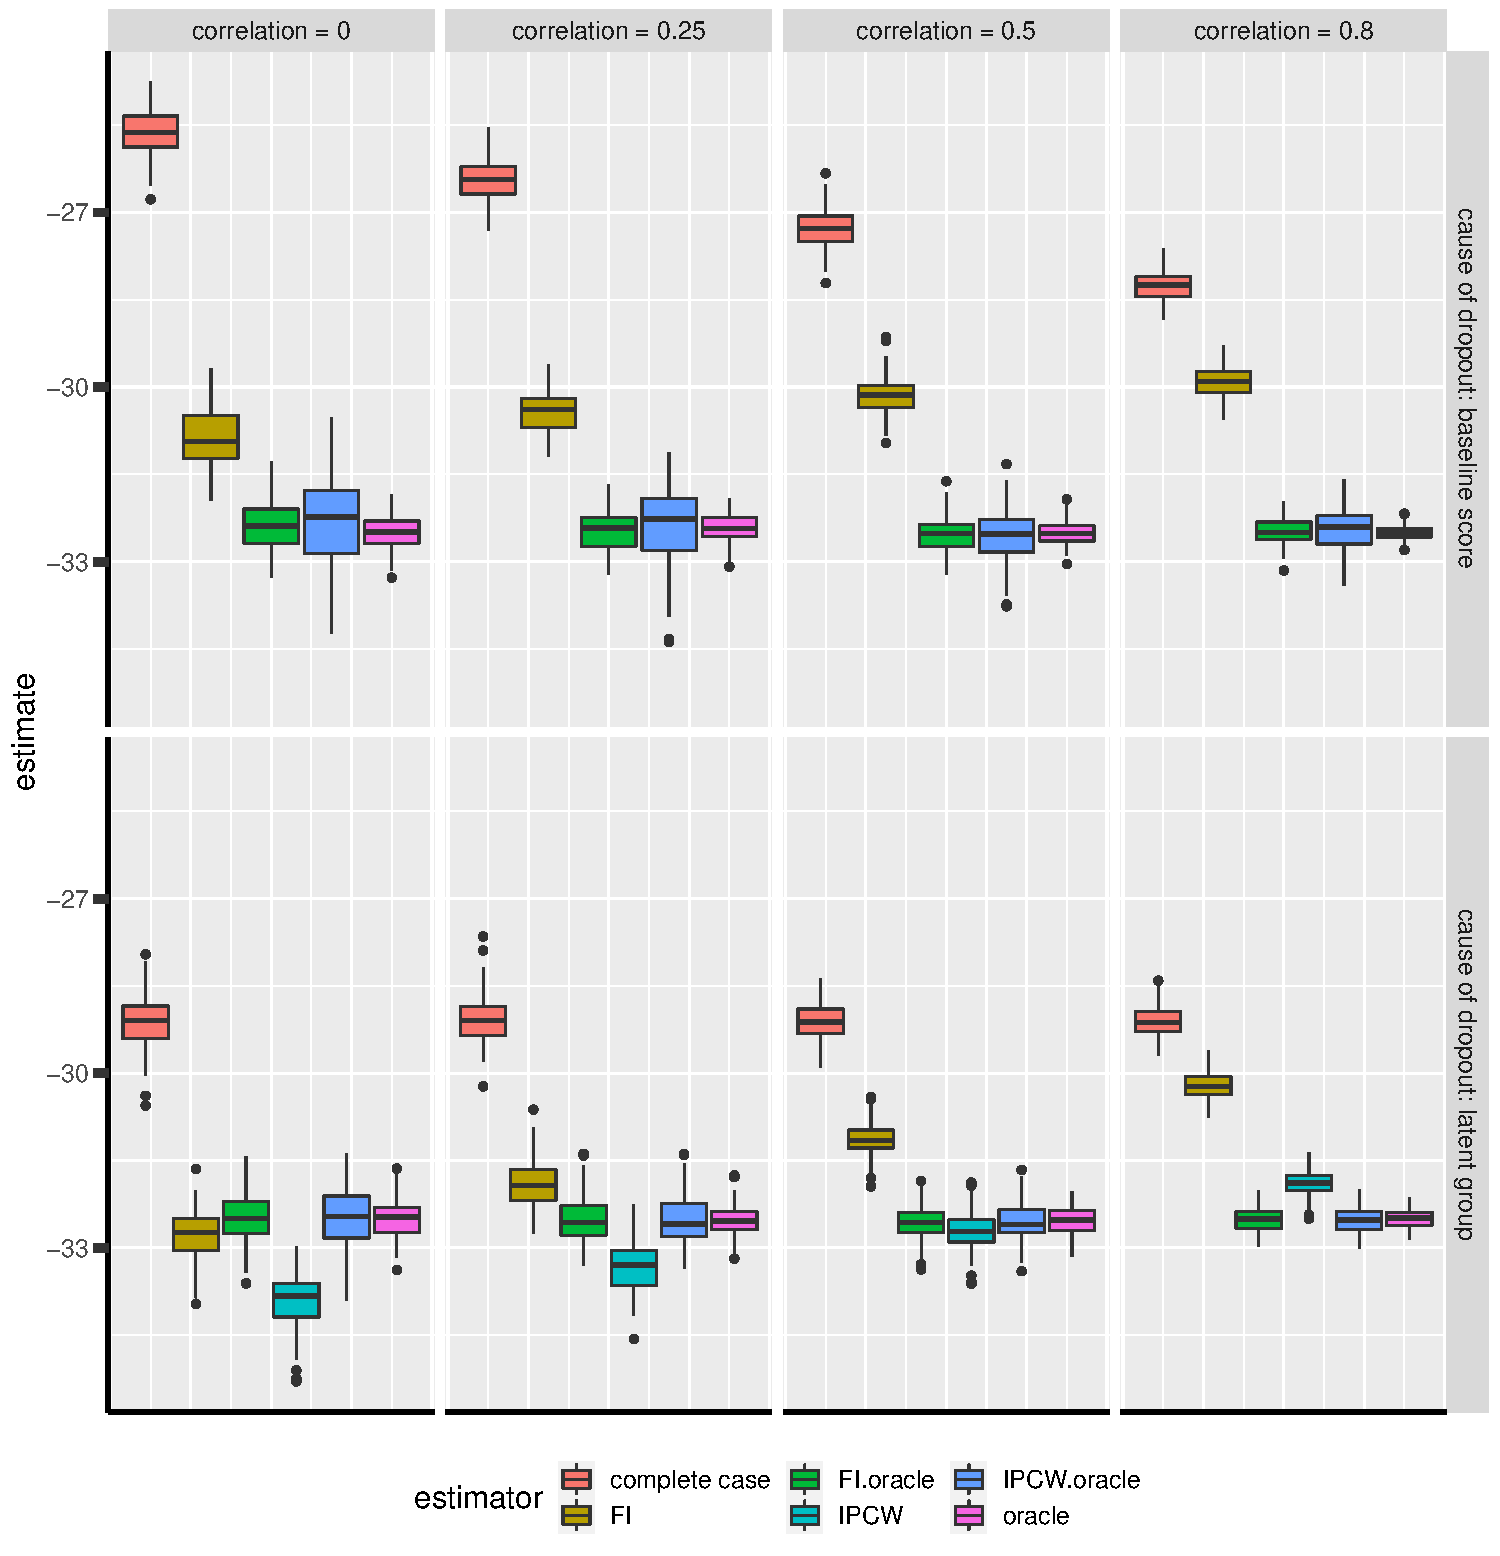
\includegraphics[width=\textwidth]{./figures/simStudy-bias.pdf}
\caption{\label{fig:simulation}Results of the simulation study for a sample size of 1000 using 100 datasets.}
\end{figure}
\end{document}